\chapter{Pruebas y rendimiento}\label{chapter4}
En los siguientes apartados vamos a mostrar el procedimiento seguido para validar y medir las capacidades de dos de las piezas más importantes de la aplicación: el componente del lienzo y la librería \texttt{multivariate-polynomial}.  Estas comprobaciones han sido una fase esencial en la evolución de la aplicación. El lienzo debe de presentar un rendimiento lo suficientemente bueno en todos los dispositivos para una buena experiencia de usuario. Esto es cierto también en el caso de la librería de polinomios, pero en su caso habrá además que comprobar que todos sus métodos y algoritmos producen resultados correctos.

\section{Lienzo}
La sección de la aplicación \texttt{Playground} mencionada en la \autoref{sec:lienzoImplem} fue ideada originalmente como un escenario de pruebas de rendimiento que no estaría en el entorno de producción, pero eventualmente su estado avanzó hasta tomar la forma actual. En su primera etapa de desarrollo, este componente solo contaba con un lienzo dibujando una escena de prueba similar a la de la \autoref{fig:resAA} con una cámara orbitando de forma continua, un medidor de su resolución, y unos interruptores con los que elegir qué algoritmos de visualización usar. Actualmente esta sección cuenta además con controles para los materiales de las primitivas y las propiedades de las luces, incluyendo color, tamaño e intensidad, y está totalmente disponible su uso al usuario. Junto a la información del rendimiento de las herramientas de desarrollador de Google Chrome, que permiten medir los FPS (fotogramas por segundo) de la aplicación, tenemos información suficiente para evaluar el rendimiento del lienzo.\newline

Se han hecho pruebas de rendimiento en dos equipos diferentes, uno de sobremesa y un portátil, cuyas características se muestran en la \autoref{fig:specs}. En ambos equipos se han probado todas las combinaciones de activación de los algoritmos de visualización de sombras y oclusión ambiental junto a valores del factor de supermuestreo $AA$ del \textit{antialiasing} entre uno (no aplicar \textit{antialiasing}) y cuatro (resolución interna dieciséis veces mayor a la mostrada), todo esto en dos configuraciones de resolución para el lienzo. En las gráficas que iremos mostrando a continuación se representan en el eje vertical los fotogramas por segundo medidos, y en el horizontal el factor de escalado del \textit{antialiasing}, pues veremos que será este factor el que más afecte al rendimiento.\newline
\begin{figure}[hb!]
    \centering
    \begin{table}[H]
\begin{tabular}{l|l|l|}
\cline{2-3}
                                        & \textbf{Sobremesa}                      & \textbf{Portátil}                               \\ \hline
\multicolumn{1}{|l|}{\textbf{GPU}}      & NVIDIA GeForce GTX 1060 6GB             & NVIDIA GeForce GTX 1650                         \\ \hline
\multicolumn{1}{|l|}{\textbf{CPU}}      & Intel(R) Core(TM) i5-8400 @ 2.80GHz & AMD Ryzen 7 4800H @ 2.90 GHz \\ \hline
\multicolumn{1}{|l|}{\textbf{RAM}}      & 8,00 GB                                 & 16,0 GB                                         \\ \hline
\multicolumn{1}{|l|}{\textbf{Pantalla}} & 2560 px $\times$ 1440 px $\times$ 144 hz               & 1920 px  $\times$ 1080 px  $\times$ 60 hz                                  \\ \hline
\end{tabular}
\end{table}
    \caption{Especificaciones de los equipos usados en las pruebas}
    \label{fig:specs}
\end{figure}

\begin{figure}[ht!]
    \centering
    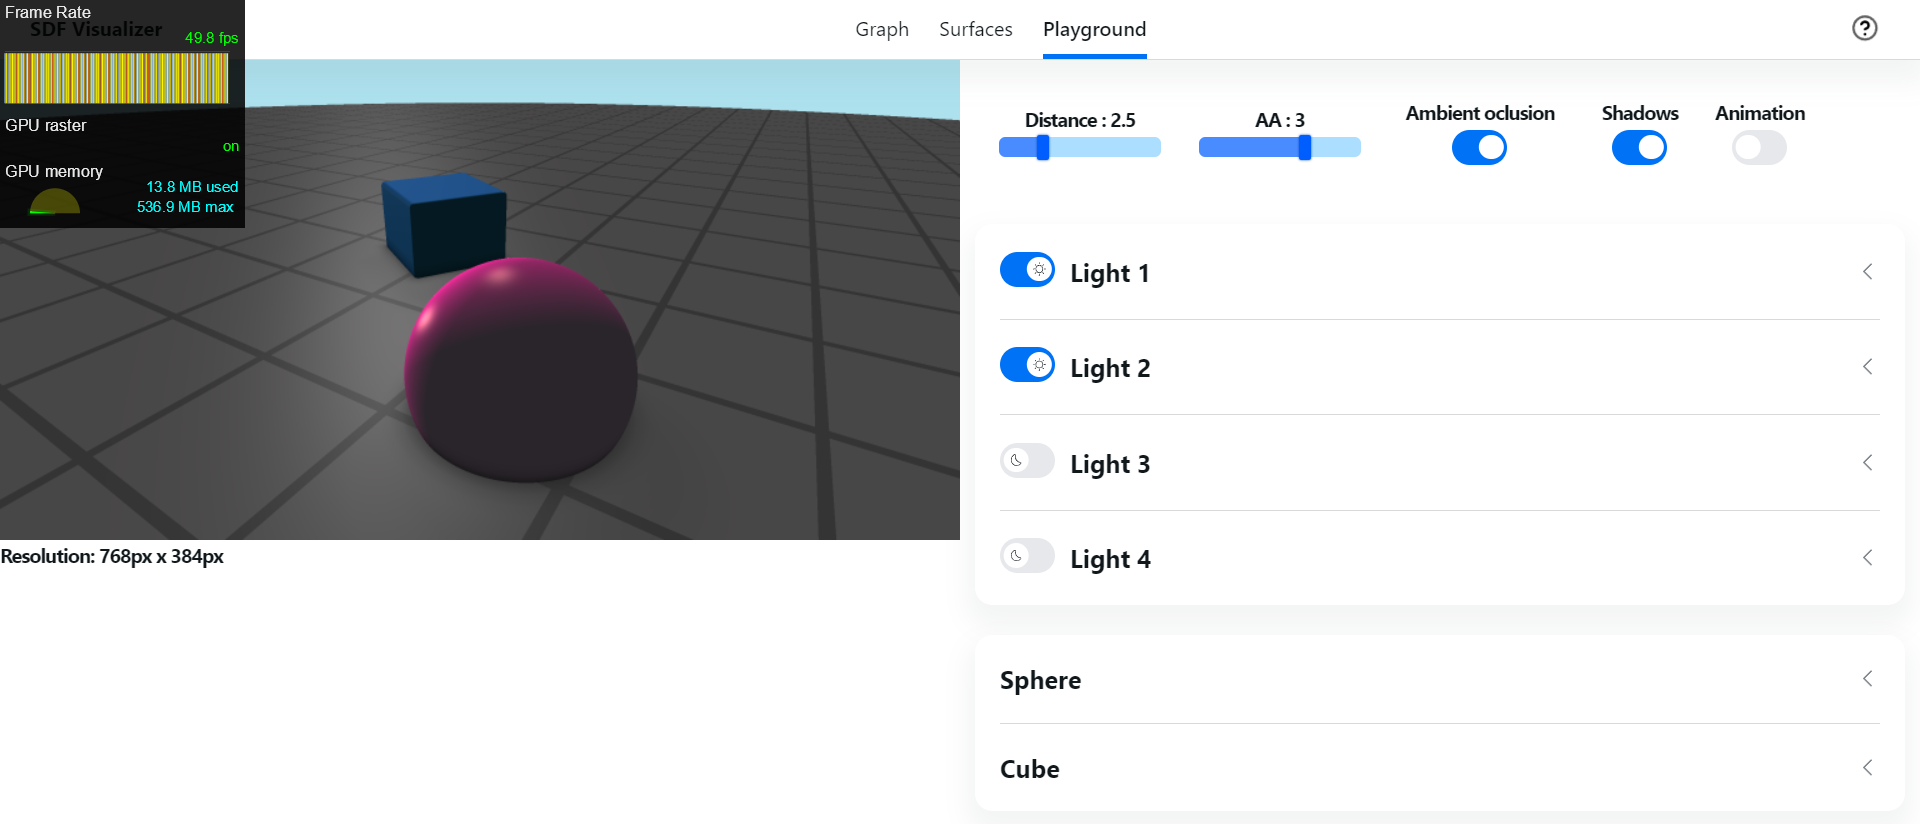
\includegraphics[width=\textwidth]{Plantilla-TFG-master/img/playground.png}
    \caption{Sección \texttt{Playground} de la aplicación usada para medir el rendimiento de esta}
\end{figure}


Empecemos estudiando el ordenador de sobremesa en su configuración de resolución más alta para el lienzo (\autoref{fig:sobreHR}). En su versión más básica (sin sombras, oclusión ambiental o \textit{antialiasing}) se obtiene un rendimiento muy alto, tanto que está limitado por la frecuencia de refresco de la pantalla, en este caso 144 Hz. Como habíamos adelantado, el algoritmo más demandante es el de \textit{antialiasing}, y cada vez que se aumenta su factor de escalado el rendimiento se reduce aproximadamente a la mitad para cualquier otra combinación de valores. Todo lo contrario ocurre con el algoritmo de oclusión ambiental, cuyo efecto en el rendimiento es prácticamente anecdótico, incluso en esta resolución tan alta. El de cálculo de sombras sin embargo sí que reduce el rendimiento en alrededor de un $25\%$ en todos los casos. De hecho, al aplicar ambos algoritmos simultáneamente se obtiene prácticamente el mismo rendimiento que aplicando solo el de sombras.\newline
\begin{figure}[ht!]
    \centering
    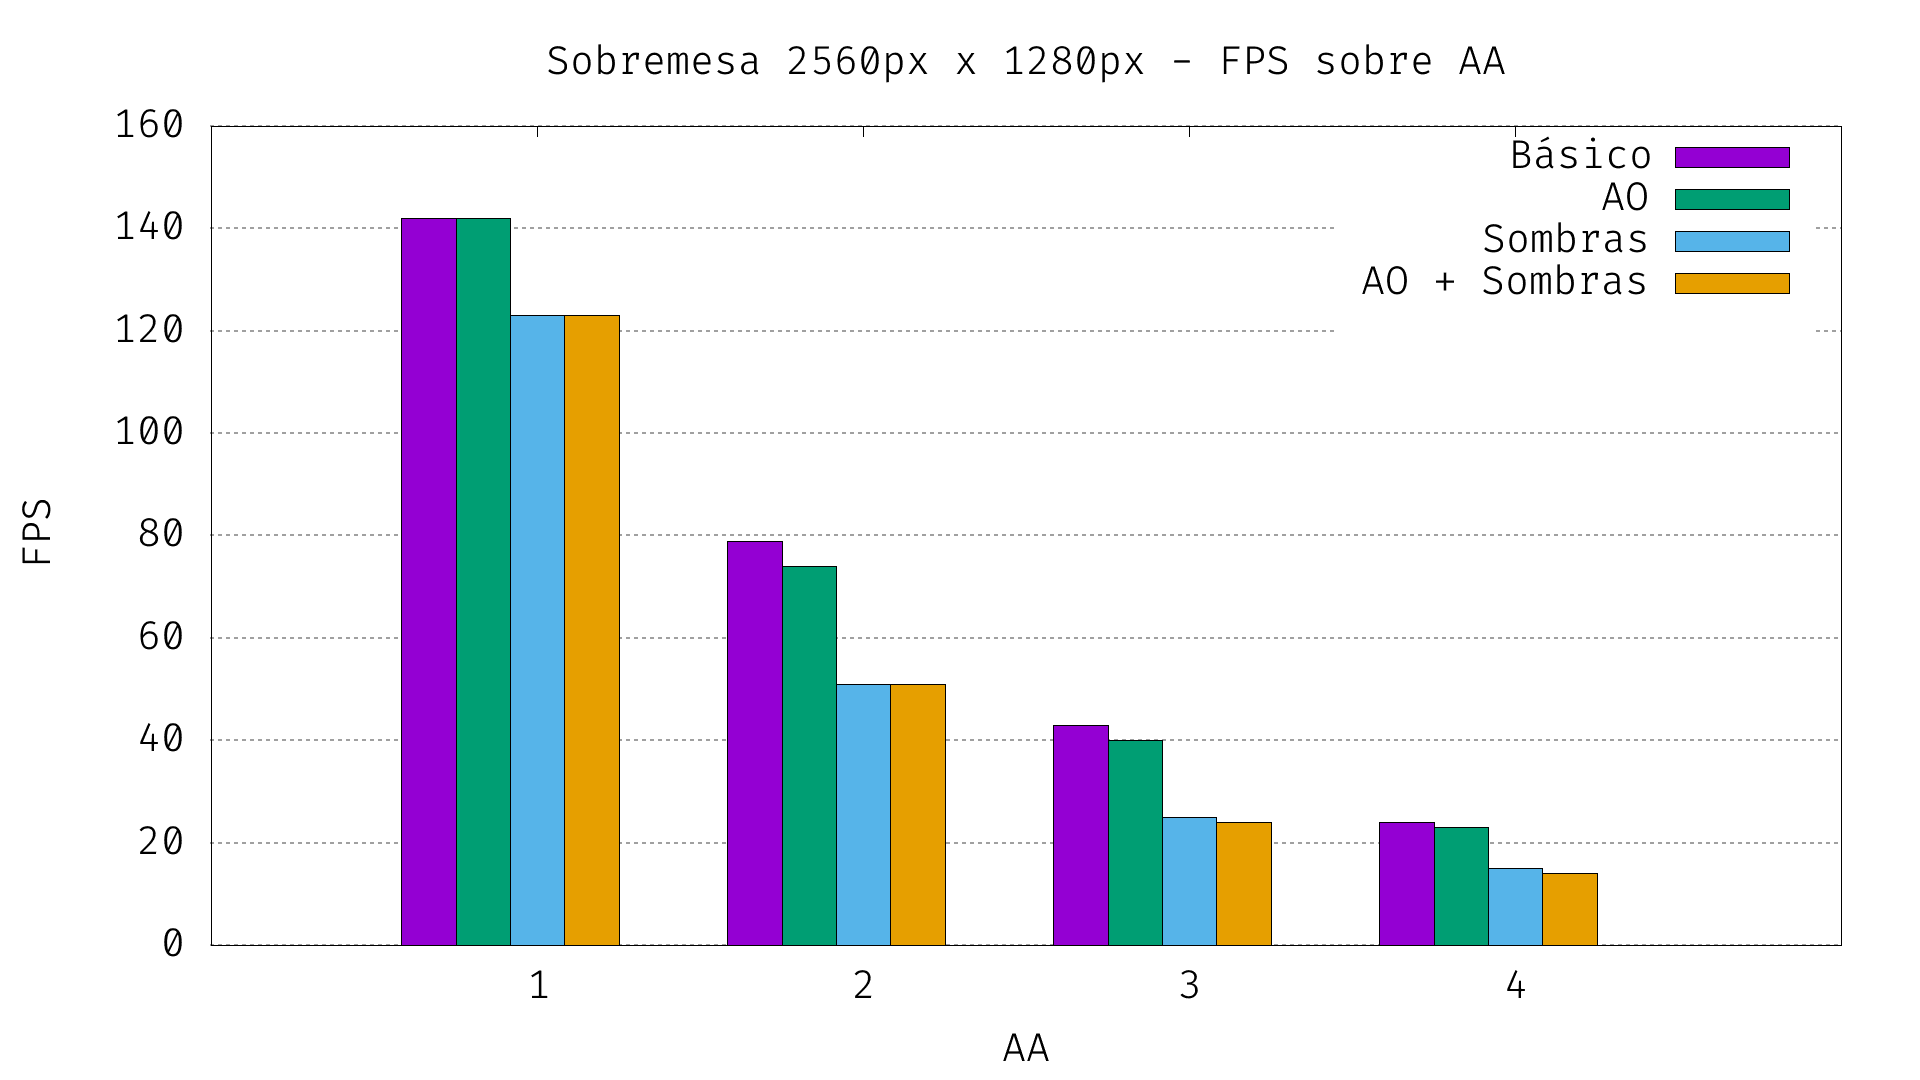
\includegraphics[width=\textwidth]{Plantilla-TFG-master/img/graficas/SobremesaHR.png}
    \caption{Rendimiento en ordenador de sobremesa con resolución alta}
    \label{fig:sobreHR}
\end{figure}

En la configuración de resolución baja obtenemos medidas en la misma línea, pero con una diferencia fundamental. Esta es que el impacto de aumentar el valor de $AA$ es menor, en concreto de un $30\%$ en lugar de un $50\%$ (también ocurre con el cálculo de sombras, que pasa a una reducción del rendimiento de un $10-15\%$). Esto es debido a que, si recordamos de la \autoref{sec:aa}, el número de rayos a trazar por cada píxel crece en función de $AA^2$, y por consiguiente reducir el número de pixels inicial disminuye también enormemente el número final de rayos. En efecto, dado que ahora trabajamos con un cuarto de la resolución anterior, el número de rayos a evaluar por píxel en esta configuración con $AA=n$ es el mismo que en la configuración de resolución alta con $AA=n-2$. A primera vista podría parecer que el rendimiento debería ser el mismo en ambos escenarios, pero en la \autoref{fig:sobreLR} podemos observar que esto no ocurre. El motivo de esto es que no todo el tiempo de renderizado se dedica a cálculos relacionados con los rayos, sino que el \textit{shader} también emplea otra parte de este tiempo en cálculos que se hacen una única vez por píxel (independientemente de $AA$), y otra en tiempos fijos (independientes de $AA$ y del número de pixels).
\begin{table}[!ht]
    \centering
    \begin{tabular}{|l|l|l|l|l|}
        \hline
        & $\boldsymbol{AA=1}$ & $\boldsymbol{AA=2}$ & $\boldsymbol{AA=3}$ & $\boldsymbol{AA=4}$ \\ \hline
        \textbf{2560 px $\times$ 1280 px} & $3,2768 \times 10^6$  & $6,5536  \times 10^6$ & $13,1072  \times 10^6$ & $26,2144 \times 10^6$ \\ \hline
        \textbf{1280 px $\times$ 640 px} & $0,8192  \times 10^6$ & $1,6384  \times 10^6$  & $3,2768 \times 10^6$ &  $6,5536  \times 10^6$ \\ \hline
    \end{tabular}
    \caption{Rayos a trazar en función de la resolución inicial y $AA$}
\end{table}

Este decremento tan sustancial en el número de rayos hace que obtengamos una gran mejora en el rendimiento, como era de esperar, y desactivando las sombras obtenemos 144 Hz incluso con $AA=2$. Es fácil suponer por tanto que para $AA=1$ las medidas están claramente limitadas por la tasa de refresco del monitor y serían mucho mayores al valor medido, de en torno a los 200 Hz si asumimos que el rendimiento se reduce en un $30\%$ al aumentar $AA$ y que para $AA=2$ las medidas obtenidas no están siendo limitadas.\newline
\begin{figure}[ht!]
    \centering
    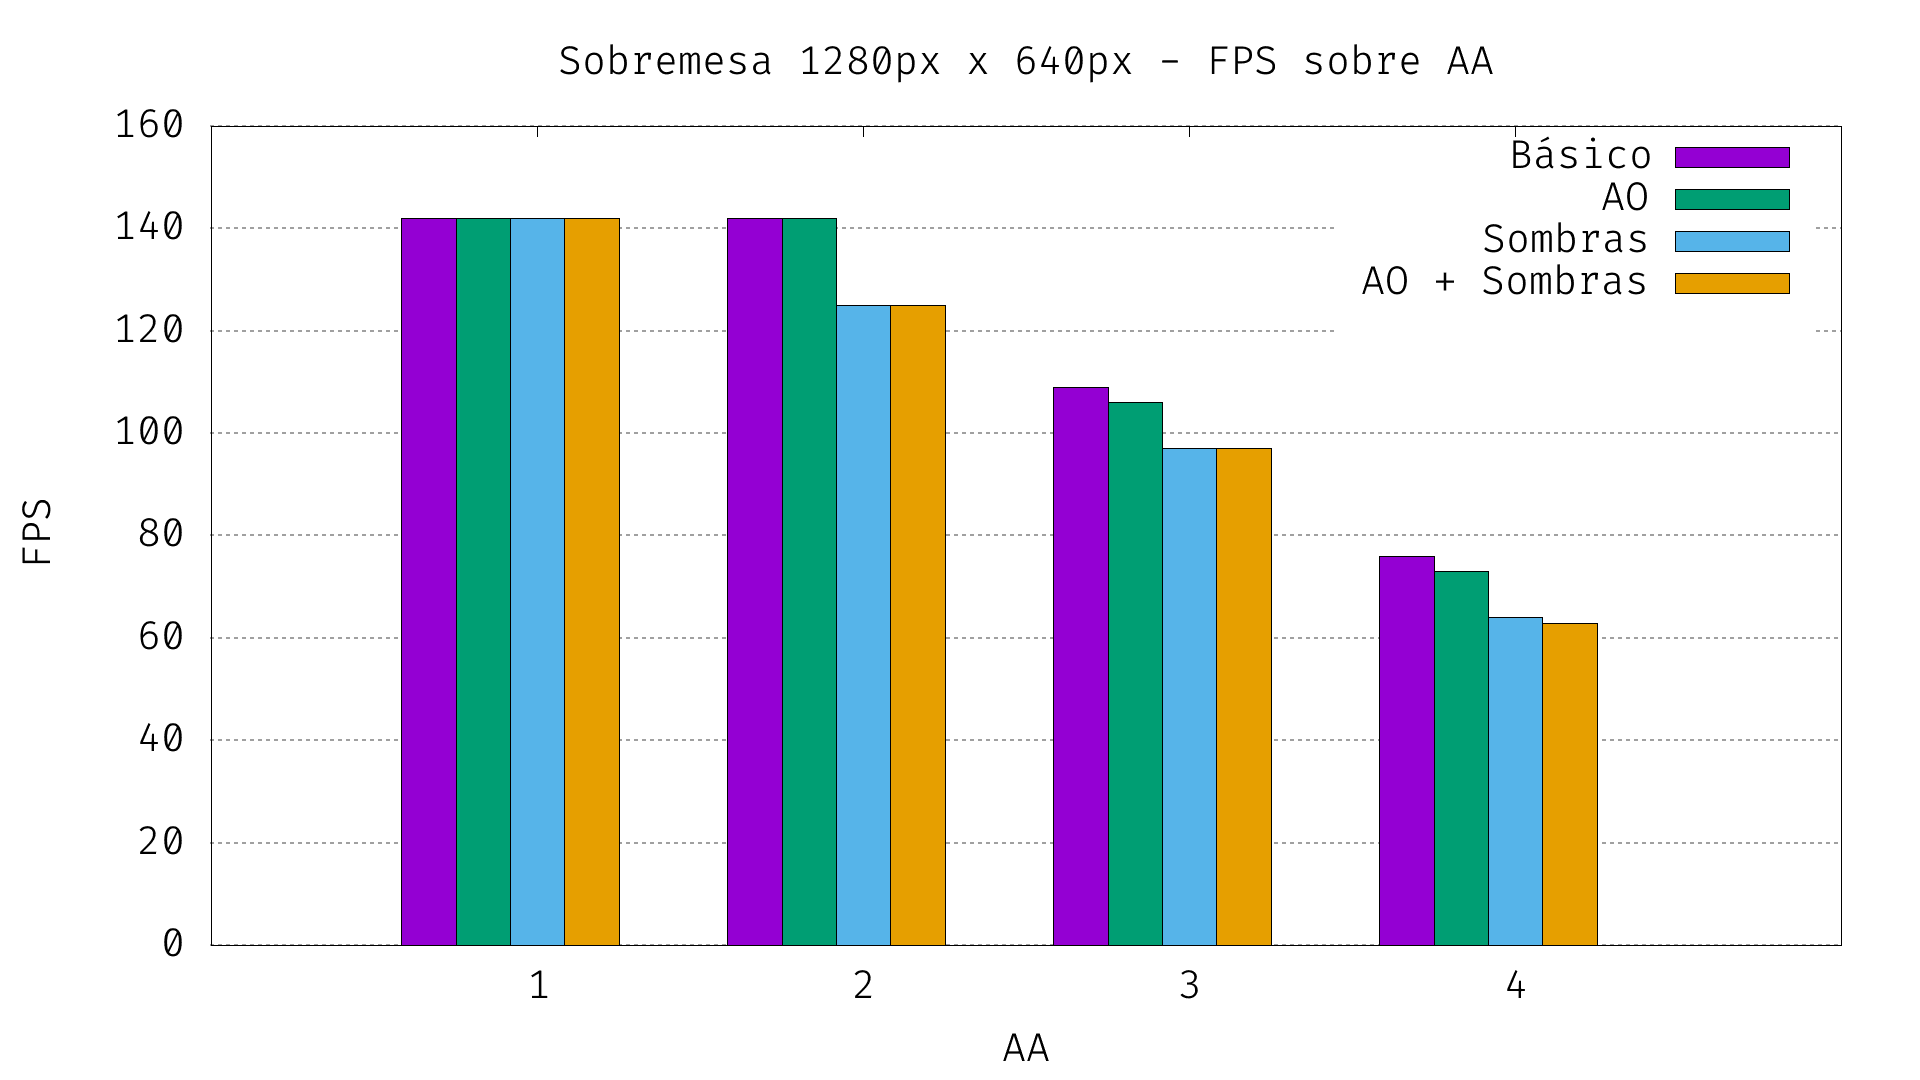
\includegraphics[width=\textwidth]{Plantilla-TFG-master/img/graficas/SobremesaLR.png}
    \caption{Rendimiento en ordenador de sobremesa con resolución baja}
    \label{fig:sobreLR}
\end{figure}

A vista de las gráficas anteriores podríamos pensar que usar $AA=3$ es una buena opción, pues obtenemos unas medidas bastante buenas de FPS. En concreto, en resolución baja obtenemos alrededor de 100 FPS, y con resolución alta llegamos a conseguir 40 FPS. En ambos casos obtenemos valores por encima de los 30 FPS, que suele ser considerado el mínimo para una buena experiencia interactiva. Sin embargo, hay que tener en cuenta que hay otros factores además de los fotogramas por segundo que influyen en la fluidez de la imagen, entre los que destaca el \textit{frametime}.\newline

El \textbf{\textit{frametime}} es el tiempo en milisegundos que se tarda en renderizar cada fotograma, incluyendo tanto los cálculos visuales como otros adicionales (motor de físicas, postprocesado, etc.). Queremos que este tiempo sea lo más estable posible a lo largo de la ejecución del programa, pues representa cada cuanto tiempo se nos presenta un fotograma nuevo en pantalla. Así, si el \textit{frametime} fluctúa mucho tendremos la sensación de que la imagen no es fluida independientemente del número de fotogramas por segundo que se muestren, ya que para el cálculo de estos solo se tiene en cuenta el numero final de fotogramas presentados. Por ejemplo, en una aplicación a 60 FPS, querríamos que el \textit{frametime} fuera de 
\begin{equation*}
   frametime = \frac{\cancel{1s}}{60 \text{ fotogramas}}\cdot \frac{1000 ms}{\cancel{1s}} = \frac{16,667 ms}{\text{fotograma}}.  
\end{equation*}
\begin{figure}[!ht]
    \centering
    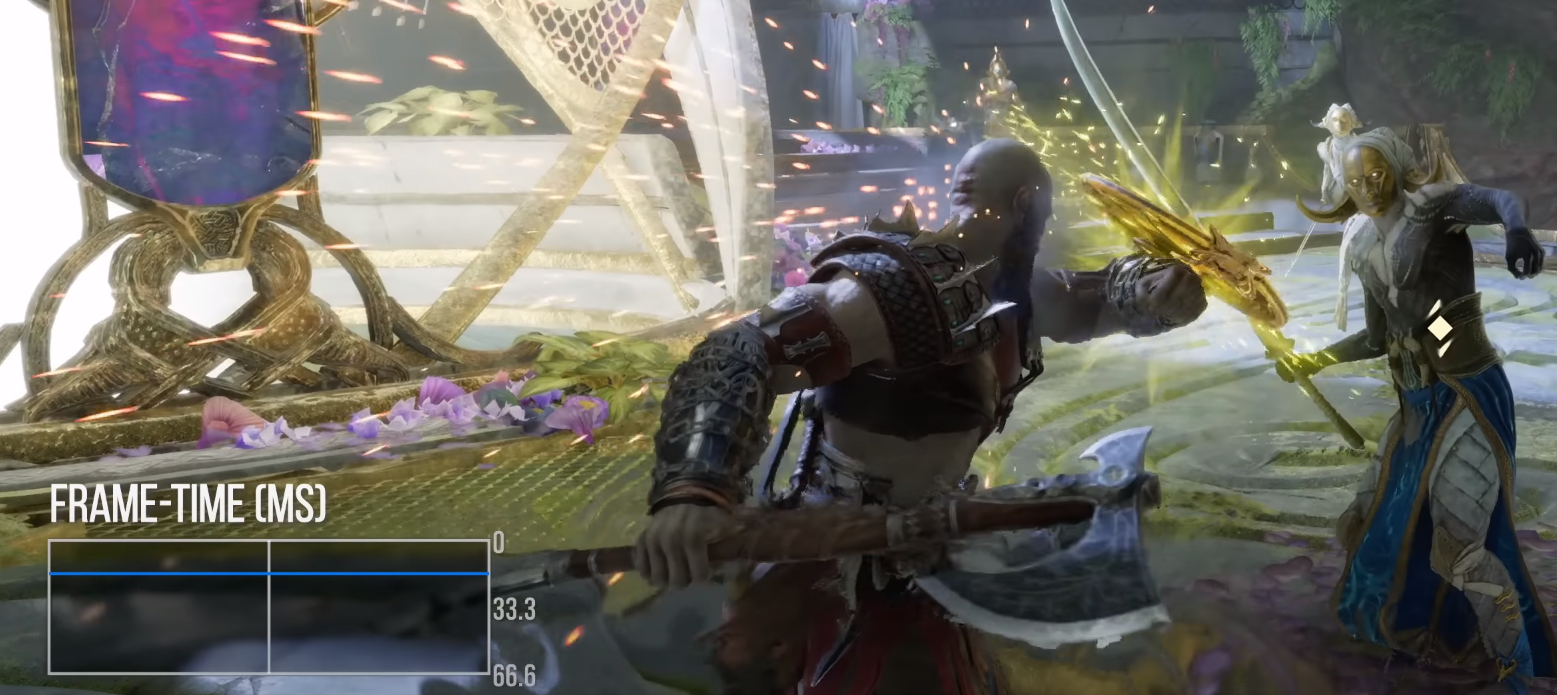
\includegraphics[width=\textwidth]{Plantilla-TFG-master/img/gow.png}
    \caption{Videojuego God of War: Ragnarök obteniendo un \textit{frametime} estable de 16.667 ms en PS5 \cite{gow}}
\end{figure}

Las herramientas de desarrollador de Google Chrome permiten también medir el \textit{frametime} de nuestra aplicación. Para valores de $AA$ menores a dos obtenemos una gráfica totalmente plana, indicando que el \textit{frametime} es muy estable, y en consecuencia el movimiento de la cámara del lienzo se percibe fluido. En cambio, a partir del valor $AA=3$ empezamos a obtener una gráfica con muchos picos, a pesar de que estemos obteniendo un gran número de fotogramas por segundo, como muestra la \autoref{fig:frametime}. Podemos afirmar por tanto que el valor de $AA=2$ es la mejor elección en general, pues nos proporciona una imagen mucho más nítida a la que obtendríamos sin \textit{antialiasing} sin sacrificar la fluidez que espera el usuario.\newline
\begin{figure}[!h]
     \begin{minipage}[c]{0.4\linewidth}
        \centering
        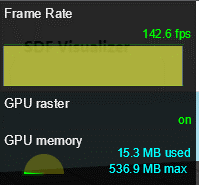
\includegraphics[width=0.98\textwidth]{Plantilla-TFG-master/img/graficas/frametimeG.png}
        \caption{$AA=2$}
     \end{minipage}
     \hfill
     \begin{minipage}[c]{0.4\linewidth}
        \centering
        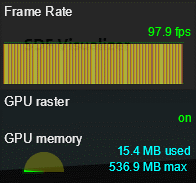
\includegraphics[width=0.98\textwidth]{Plantilla-TFG-master/img/graficas/frametimeB.png}
        \caption{$AA=3$}
     \end{minipage}
     \caption{Gráficas de \textit{frametime} según el valor de $AA$}
     \label{fig:frametime}
\end{figure}

En el ordenador portátil (\autoref{fig:laptop}) medimos un comportamiento similar al del equipo de sobremesa, con la diferencia de que las medidas obtenidas decrecen proporcionalmente al peor \textit{hardware}. En particular, ahora la pantalla ahora tiene una tasa de refresco y resolución menores. Con resolución alta (que en realidad es tan solo un poco mayor que la resolución baja del ordenador de sobremesa) obtenemos buenos resultados con hasta $AA=2$, pero si seguimos aumentando el factor de escalado obtenemos FPS muy bajos, que aún sin tener en cuenta la inestabilidad del \textit{frametime}, harían la aplicación inutilizable. Con resolución baja obtenemos resultados mucho mejores, y se ve claramente la limitación en el refresco de la pantalla a 60 Hz, pues obtenemos 60 FPS tanto con $AA=1$ como $AA=2$ con sombras y oclusión ambiental. Con $AA=3$ obtenemos también buen rendimiento, pero el problema del \textit{frametime} persiste, luego sigue siendo recomendable quedarnos con $AA=2$.\newline
\begin{figure}[!ht]
     \begin{minipage}[c]{\linewidth}
        \centering
        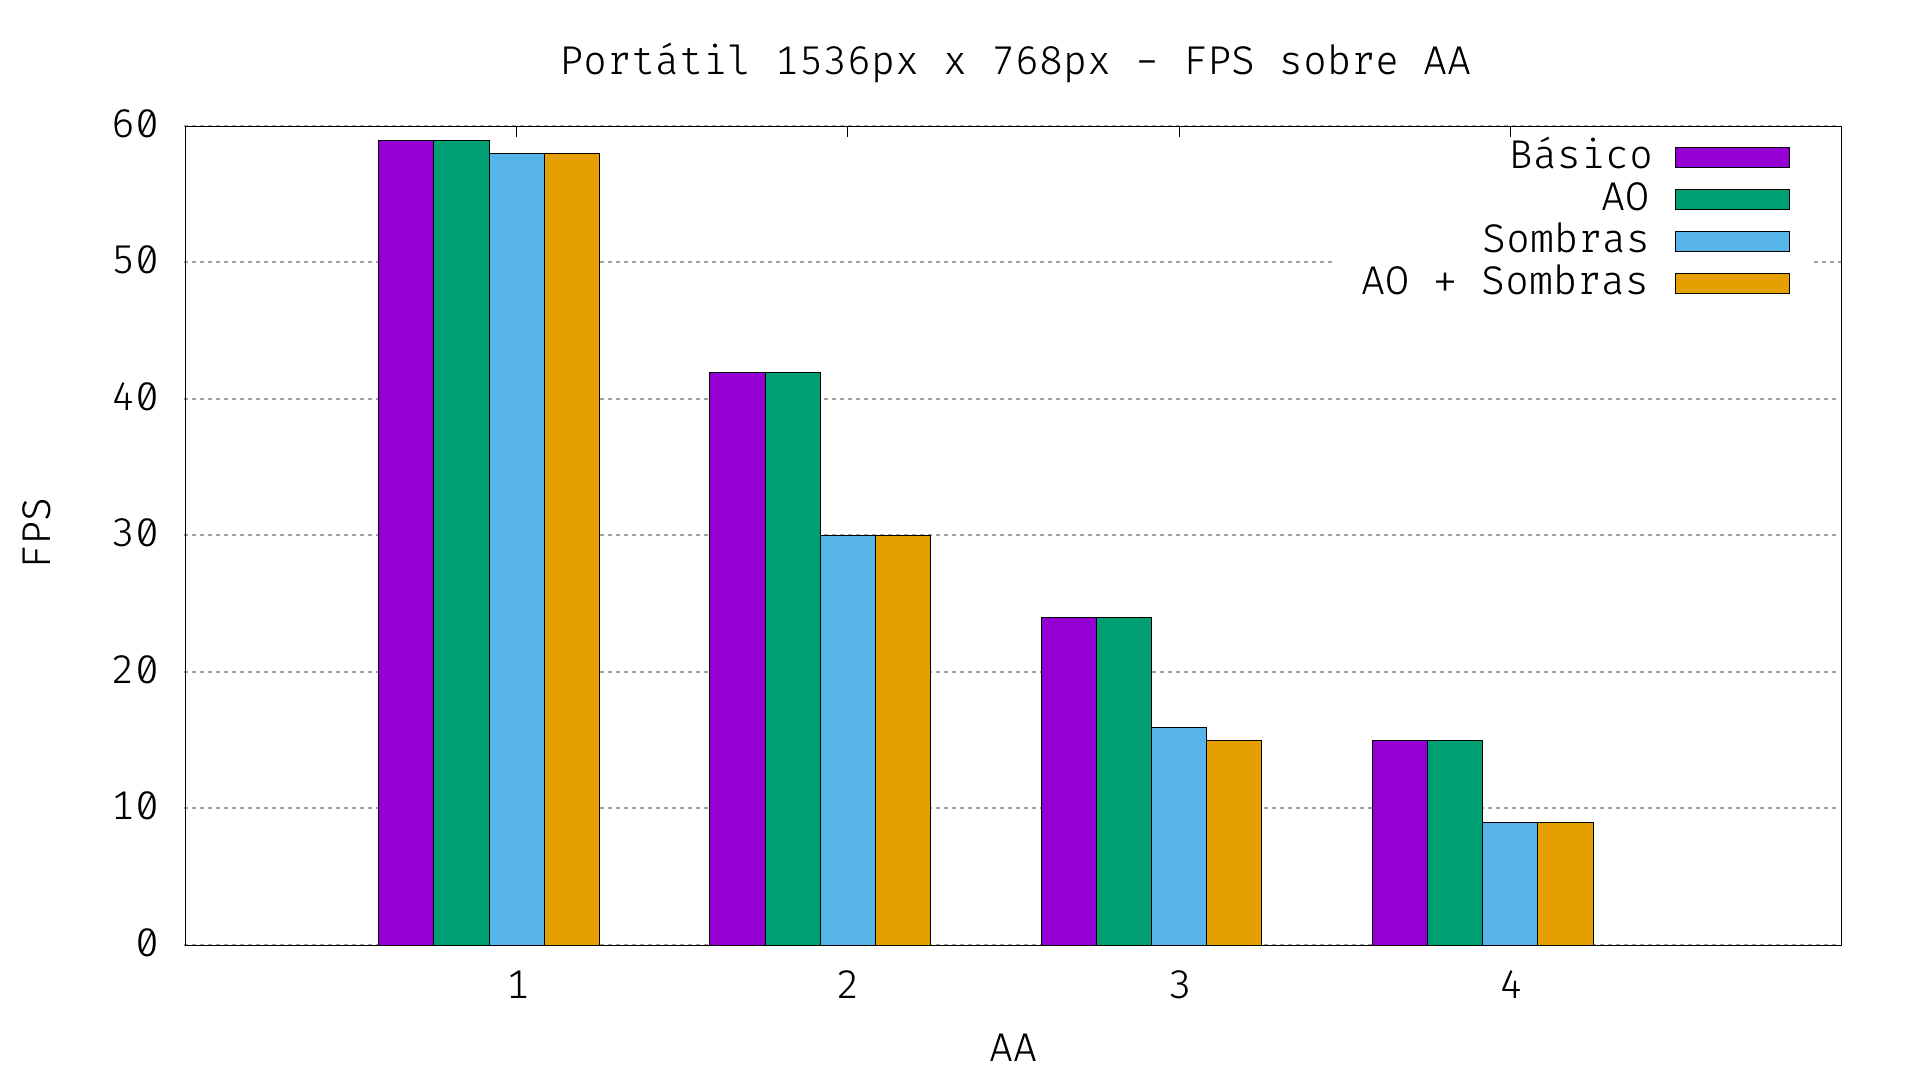
\includegraphics[width=0.98\textwidth]{Plantilla-TFG-master/img/graficas/LaptopHR.png}
        \caption{Resolución alta}
     \end{minipage}
     \begin{minipage}[c]{\linewidth}
        \centering
        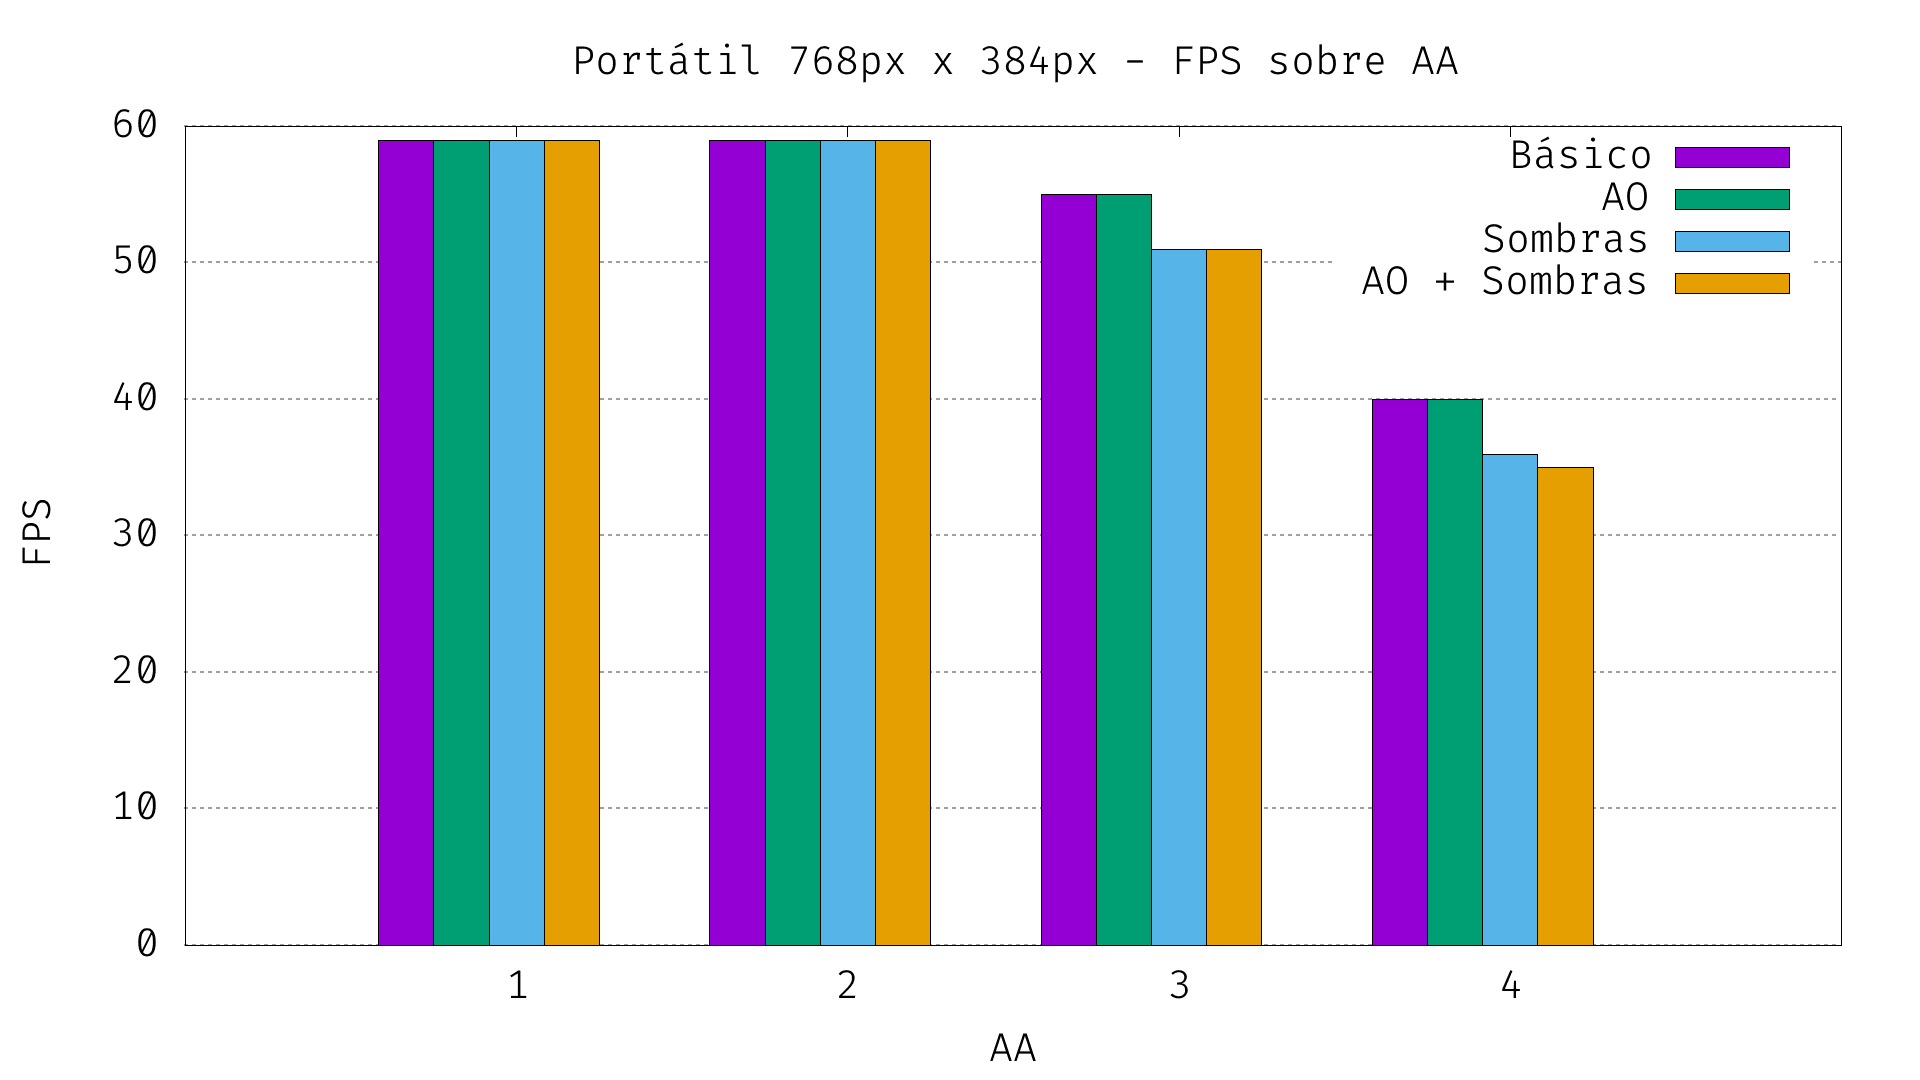
\includegraphics[width=0.98\textwidth]{Plantilla-TFG-master/img/graficas/LaptopLR.png}
        \caption{Resolución baja}
     \end{minipage}
     \caption{Rendimiento en ordenador portátil}
     \label{fig:laptop}
\end{figure}

A la vista de los resultados presentados, podemos concluir que la configuración más óptima para proporcionar una buena experiencia al usuario, tanto en rendimiento como en calidad visual, es tomar $AA=2$ y activar la oclusión ambiental. En lo que respecta a las sombras, puede ser necesario tener que desactivarlas si se trabaja en un equipo con prestaciones muy bajas, pero en general son una opción viable y añaden mucha riqueza a la escena. Esta es precisamente la configuración de los lienzos que aparecen en cada nodo del editor de nodos. Uno podría pensar que en un caso de uso complejo del editor como fue el mostrado en la \autoref{fig:ejemploCSG}, el rendimiento se vería afectado al contar con tantas instancias del lienzo. Sin embargo, nada más lejos de la realidad, ya que se obtiene un rendimiento estable al mayor número de FPS que la pantalla permite en ambos equipos. ¿Cómo es esto posible? Principalmente por dos motivos.
\begin{enumerate}
    \item Los lienzos presentes en los nodos tienen una resolución típica mucho menor a la usada en las pruebas.
    \item El lienzo no calcula nuevos fotogramas a no ser que sea necesario. Es por este motivo que en el lienzo de prueba la cámara se movía continuamente, pero en el caso del editor la cámara está fija a no ser que el usuario interactúe con ella mediante el ratón. Esto hace que en cada momento como mucho habrá un solo lienzo que se esté actualizando continuamente, mientras que el resto estarán en un estado de reposo.
\end{enumerate}

\section{Librería de polinomios en varias variables}\label{sec:libreria}
Dado que las clases que conforman la librería tienen un alto grado de dependencia entre sí, primero se desarrolló \texttt{Monomial}, después \texttt{Polynomial}, y finalmente \texttt{Ideal}. Durante el desarrollo de todas ellas se fueron generando tests para comprobar su correcto funcionamiento, desde los métodos más básicos hasta comprobaciones de seguridad en casos extremos. Las principales ventajas que nos ha aportado esta forma de trabajar son las siguientes.
\begin{itemize}
    \item Al trabajar, por ejemplo, sobre la clase \texttt{Polynomial}, al ya habernos cerciorado de que \texttt{Monomial} funciona correctamente, podemos estar seguros de que los fallos que nos encontremos estarán dentro de esta nueva clase y enfocar nuestros esfuerzos en consecuencia.
    \item En varias ocasiones se introdujeron cambios de importancia en alguna de las clases, por ejemplo cambiar el tipo del atributo \texttt{coef} de \texttt{Monomial} de \texttt{number} a \texttt{Fraction}. Al contar con los tests podemos comprobar de forma rápida que todo sigue funcionando correctamente y de forma transparente al resto de componentes que la usen.
\end{itemize}

Para la generación de los tests se ha usado MochaJS \cite{mocha}, que también nos permite medir el rendimiento de los tests que deseemos. Los tests se encuentran disponibles en el mismo repositorio que el de la librería. Los que comprueban los métodos básicos de las clases \texttt{Monomial} y \texttt{Polynomial}, tales como suma, producto, comparaciones o inserción de variables, se encuentran en los archivos \texttt{tests/monomial.ts} y \texttt{tests/polynomial.ts}, y no requieren mucha explicación. Sí son mas interesantes otros dos archivos de tests adicionales, uno de \texttt{Polynomial} para todos los métodos relacionados con bases de Gröbner (cálculo, reducción, comprobación de si es base, etc.), y otro para \texttt{Ideal} con pruebas de aplicación del algoritmo de implicitación.\newline

En el caso de los de los tests de \texttt{Polynomial}, es de vital importancia asegurarnos de que los métodos que comprueban si un conjunto de polinomios es base de Gröbner de un ideal dado y si una base es reducida funcionan correctamente, pues usaremos estos para el resto de tests más adelante. Para ello nos hemos apoyado en el uso de SageMath, que nos proporciona métodos que nos permiten realizar estas comprobaciones fácilmente. Dado un ideal, estos son \texttt{is\_groebner}, que verifica si una lista de polinomios es base de Gröbner del ideal, y \texttt{groebner\_basis()}, que calcula una base de Gröbner reducida suya. Un ejemplo de uso de estos métodos es el siguiente.
\begin{lstlisting}[language=Python, literate={^}{$\textasciicircum$}1]
    x,y,z = QQ['x,y,z'].gens()
    I = ideal(x^5 + y^4 + z^3 - 1,  x^3 + y^3 + z^2 - 1)
    B = I.groebner_basis()
    B.is_groebner() # True
\end{lstlisting}
Una vez convencidos de que estos métodos de comprobación funcionan, podemos usarlos para validar los tests de las funciones que calculan y reducen bases de Gröbner. Como no tendremos que hacer las comprobaciones a mano, nos podemos permitir generar un gran número de tests, en este caso de hasta 50 ideales con conjuntos de generadores cada vez más complejos. Es esta además una buena oportunidad para empezar a realizar mediciones sobre el rendimiento de la librería. Además del tiempo de cómputo necesario para calcular todas las bases, podemos medir también el impacto que tiene el uso de los criterios de Buchberger introducidos en el \autoref{t:criterios}. Otro factor de nuestro interés es medir si la inclusión del uso de nuestra propia clase de fracciones en lugar del tipo genérico \texttt{number} tiene algún impacto en el rendimiento. En la \autoref{fig:criterios20} se muestran todas estas comparaciones sobre un conjunto de veinte ideales en el ordenador portátil (todas las pruebas de esta sección se realizarán en este equipo).\newline
\begin{figure}[!ht]
    \centering
    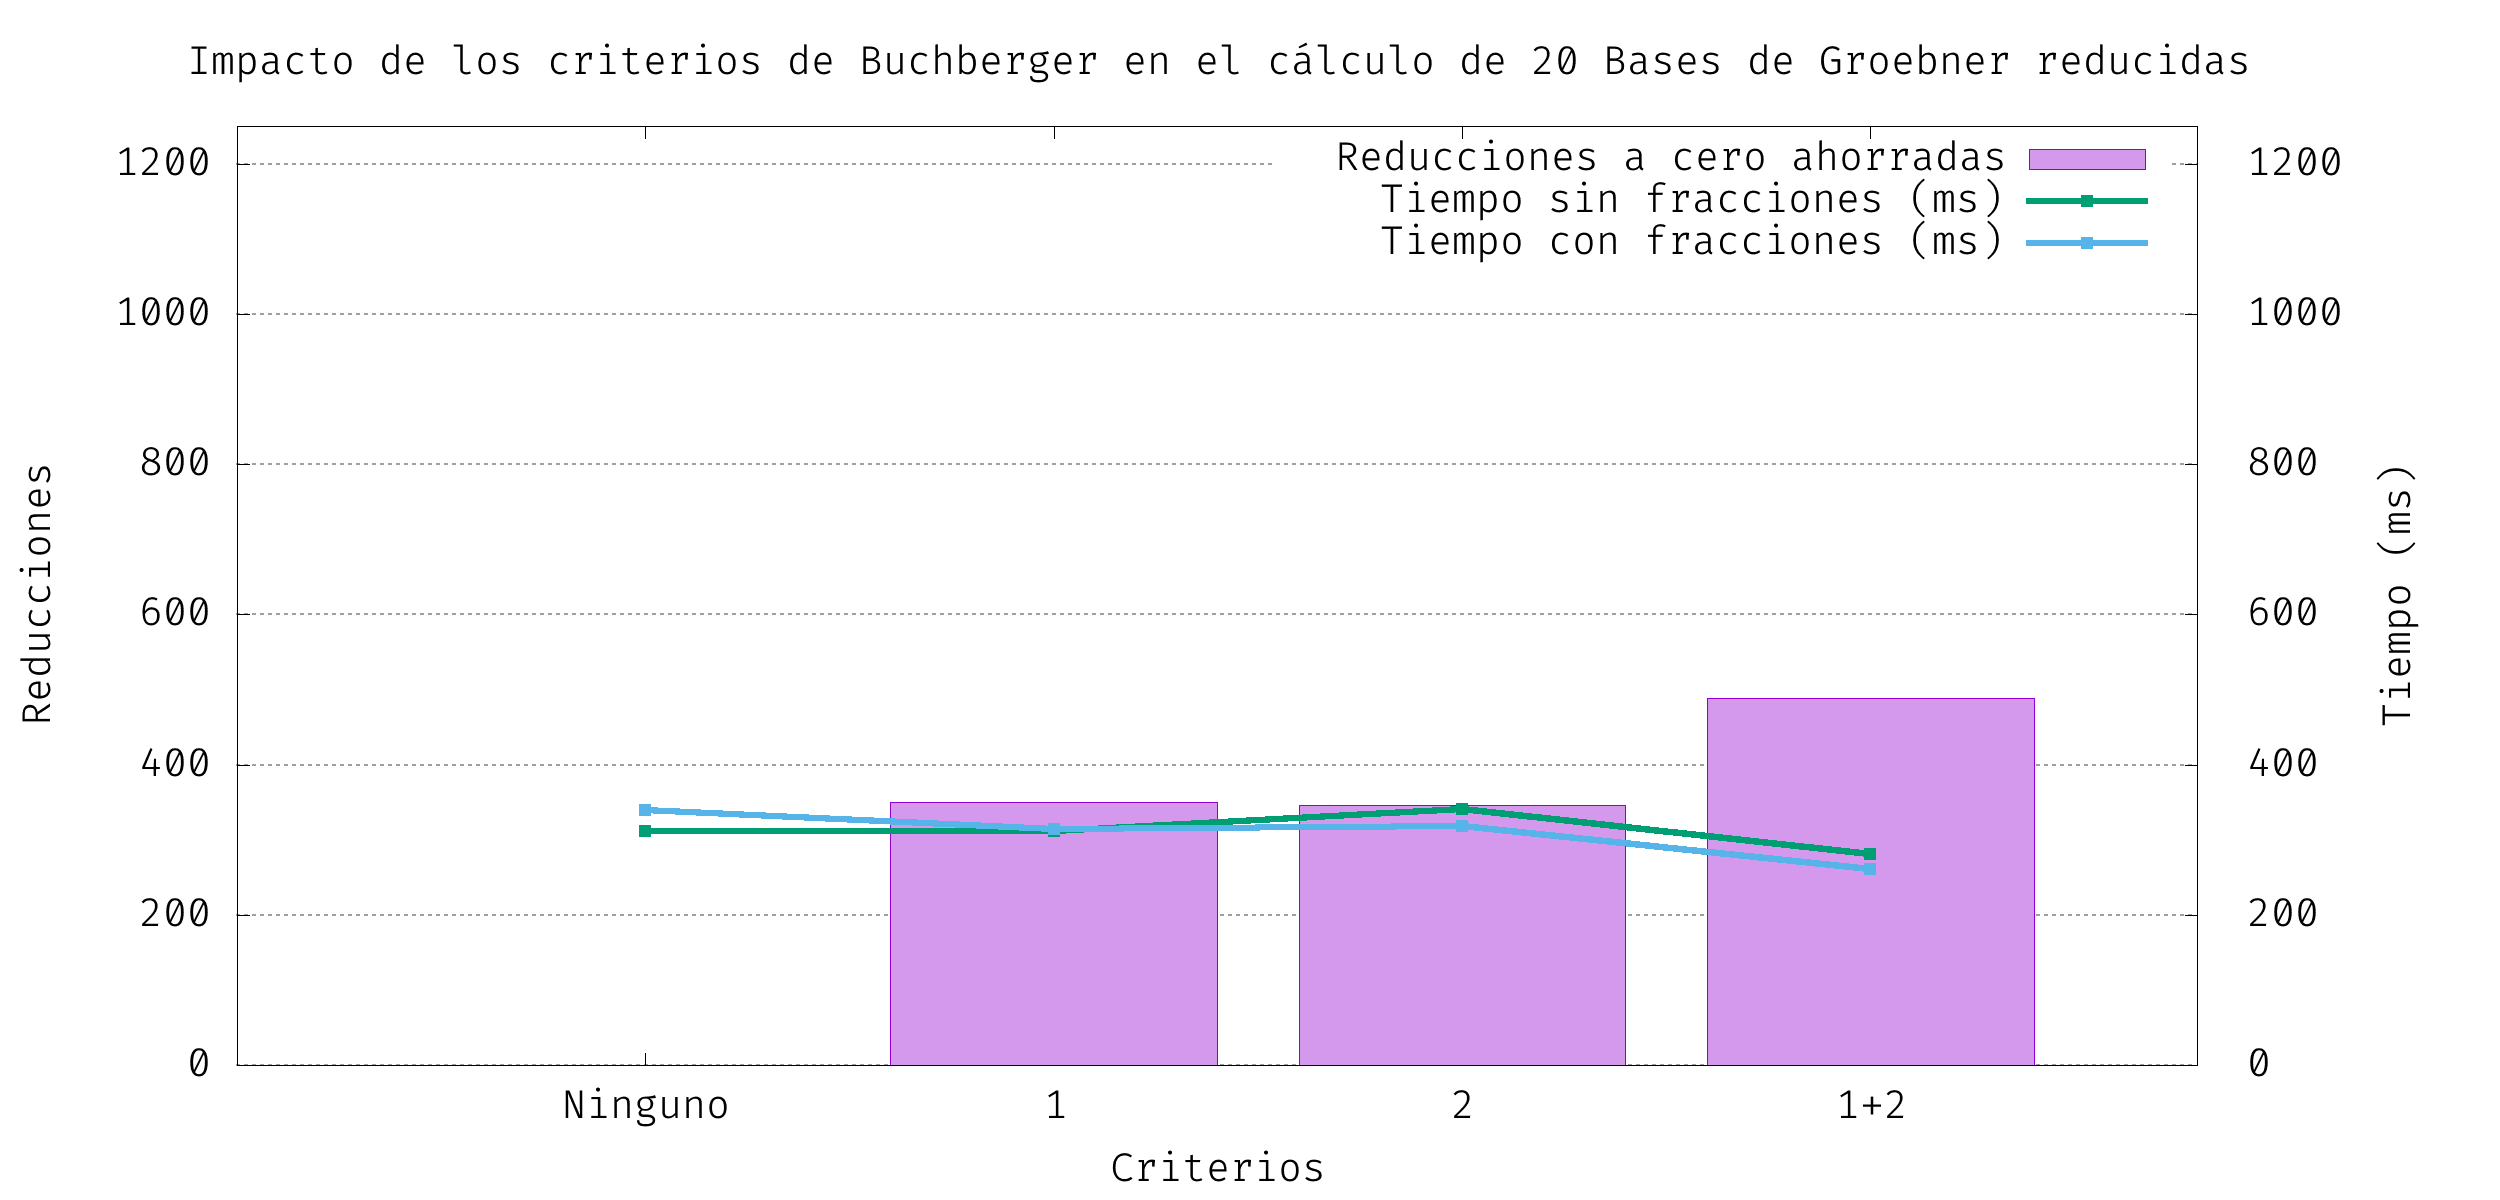
\includegraphics[width=\textwidth]{Plantilla-TFG-master/img/graficas/Criterios20-2.png}
    \caption{Rendimiento del cálculo de bases de Gröbner reducidas en una muestra de 20 ideales}
    \label{fig:criterios20}
\end{figure}

Si empezamos observando el número de reducciones a cero innecesarias, ambos criterios detectan un número similar ellas. No obstante, este número crece si ambos criterios se usan en tándem, lo cual indica que los casos que detectan uno y otro difieren, en este caso sobre un $30\%$. Como consecuencia de esto los tiempos son también menores cuando se usan ambos criterios, aunque la diferencia no es muy significativa respecto a no usar ninguno en este caso. El uso de fracciones no parece tener tampoco ninguna repercusión destacable en los tiempos obtenidos.\newline
\begin{figure}[!ht]
    \centering
    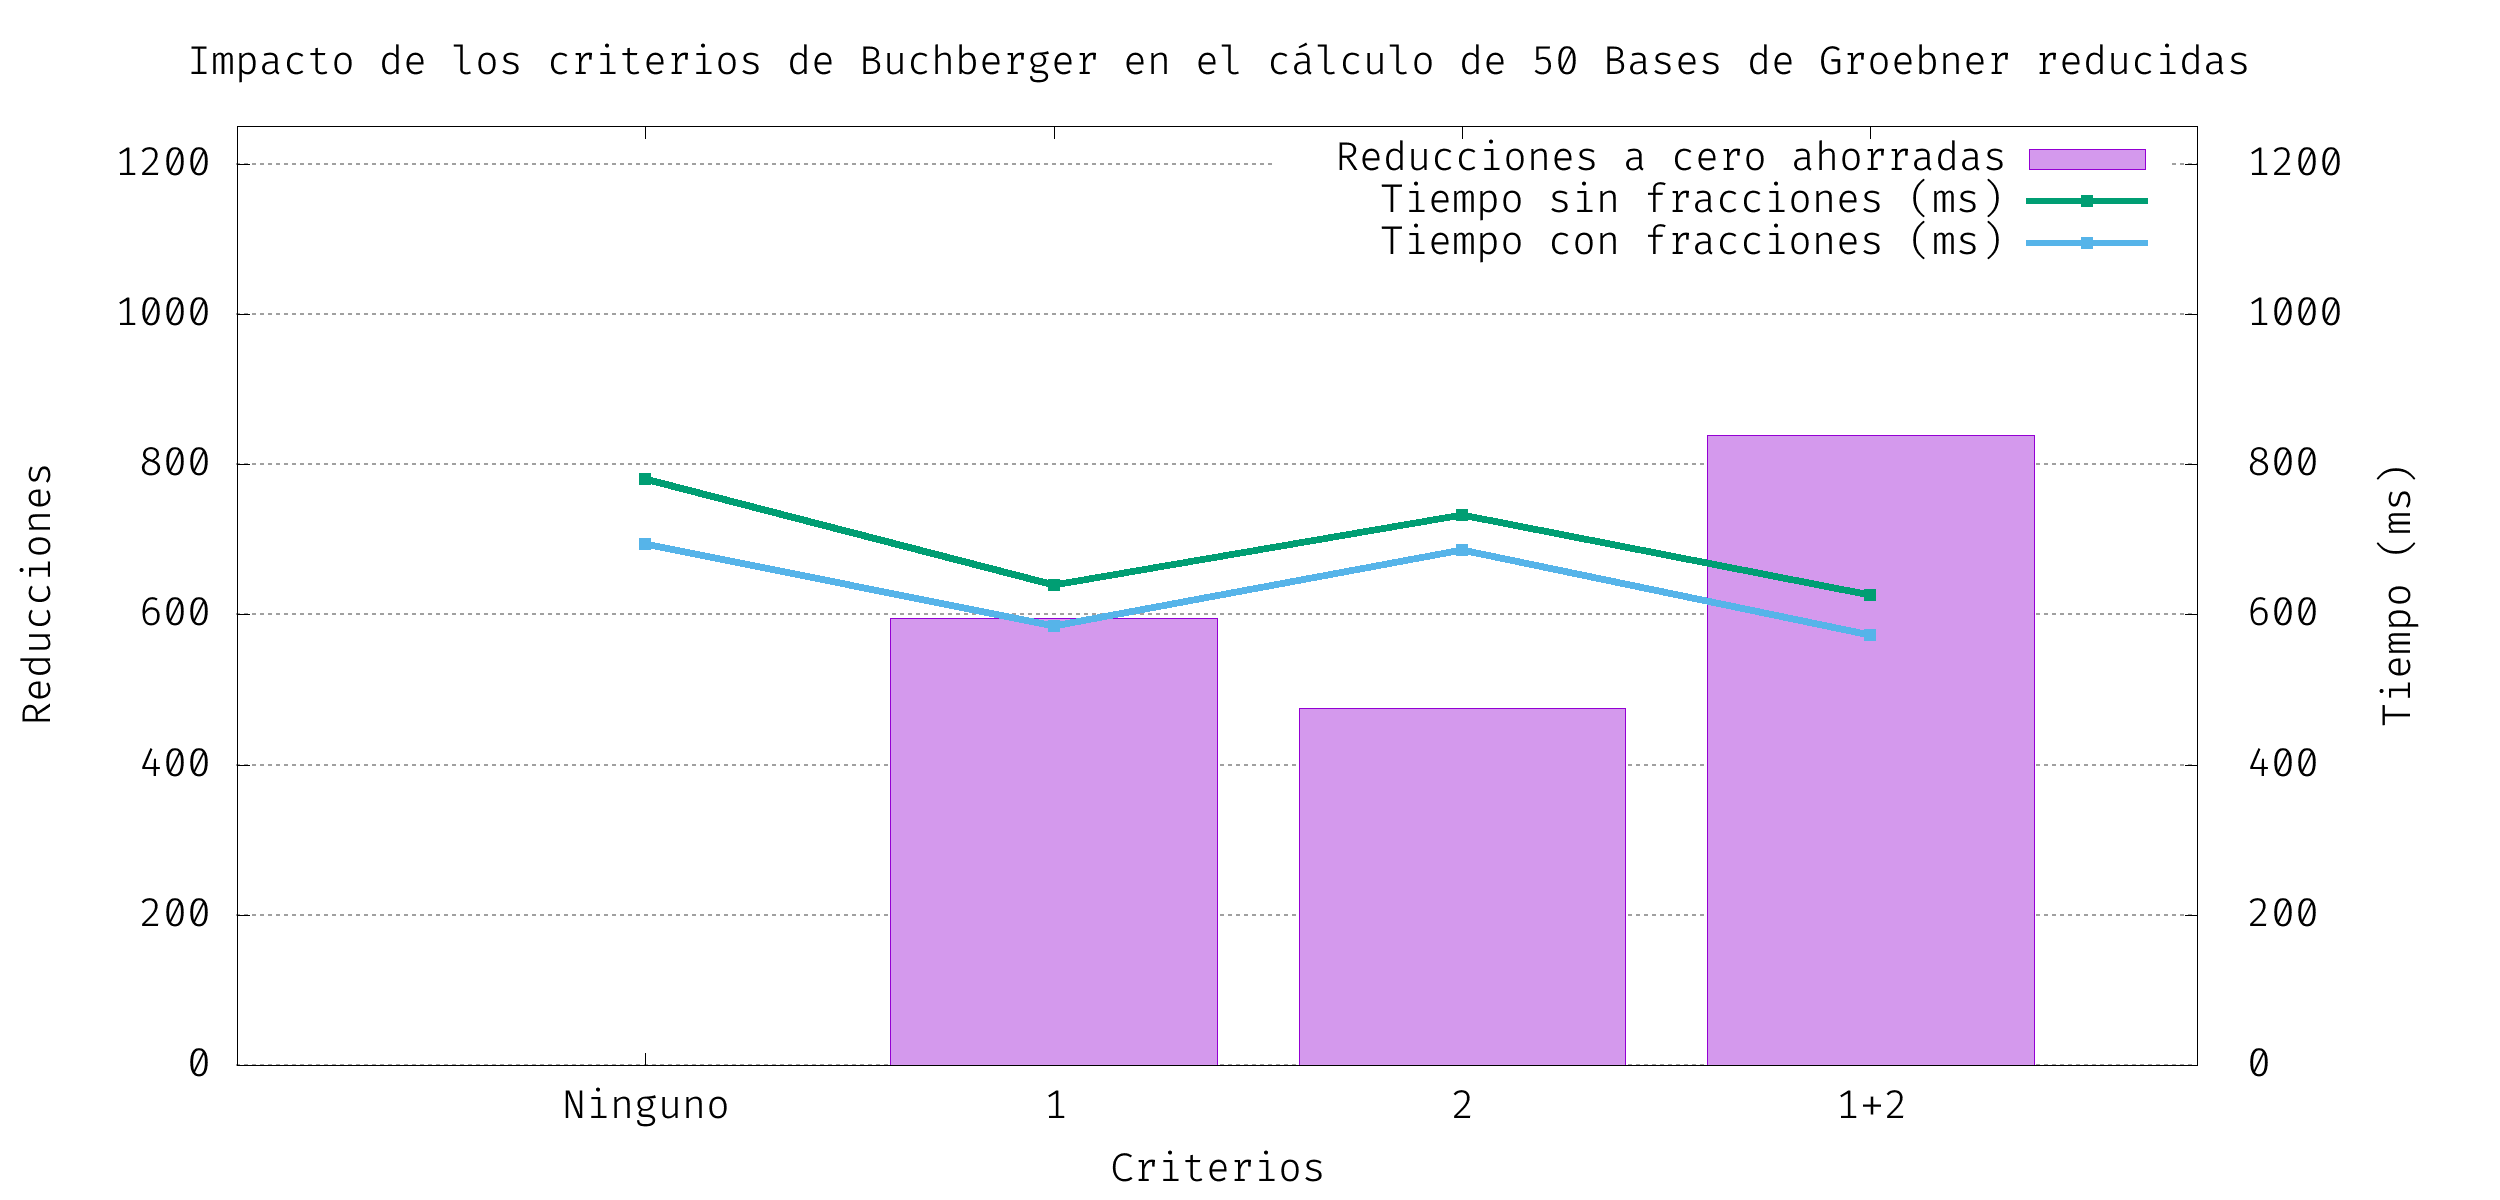
\includegraphics[width=\textwidth]{Plantilla-TFG-master/img/graficas/Criterios50-2.png}
    \caption{Rendimiento del cálculo de bases de Gröbner reducidas en una muestra de 50 ideales}
    \label{fig:criterios50}
\end{figure}

Si aumentamos el número de bases a calcular a 50 observamos que varias medidas que en la prueba anterior parecían similares ahora empiezan a distanciarse. Como primera diferencia vemos que el primer criterio ha conseguido detectar más reducciones innecesarias que el segundo, aunque este último mantiene la tendencia de detectar un $30\%$ diferentes a las del primero. Otra ventaja del primer criterio sobre el segundo es que los casos que detecta parecen ser los más útiles, ya que el tiempo total de ejecución entre usar el segundo criterio o no usar ninguno es el mismo, así como el de usar el primero o ambos a la vez. Respecto a las diferencias entre usar la clase \texttt{Fraction} o no, encontramos resultados sorprendentes, y es que usar fracciones nos proporciona mejor rendimiento que el tipo nativo \texttt{number} en todos los casos. Esta ventaja a priori tan inesperada tiene una explicación muy simple si analizamos la implementación de nuestra clase, en concreto del método de división. En él se calcula la división de dos fracciones como el producto cruzado de sus numeradores y divisores. Es decir, para dividir dos fracciones en ningún momento estamos realizando una división de flotantes, sino dos multiplicaciones. Lo que en última instancia nos importa para mejorar el rendimiento es consumir la menor cantidad posible de ciclos de reloj, y mientras que una multiplicación únicamente usa 1-2 ciclos, una división puede llegar a exceder los 24. Como en el algoritmo de división de polinomios se realizan cientos de reducciones del término líder, y en cada una de ellas dos divisiones, esta diferencia de ciclos se acumula hasta llegar a suponer una ventaja de 100 ms en nuestras pruebas.  \newline

Una vez analizado el comportamiento de la librería sobre un conjunto amplio de datos, pasamos a estudiar casos más concretos y prácticos del uso de cálculo de bases de Gröbner reducidas: la implicitación. Los tests de la clase \texttt{Ideal} buscan comprobar el correcto funcionamiento del algoritmo de implicitación implementado, para lo cual se han usado parametrizaciones racionales del plano y diversas superficies cuádricas de las que conocemos su ecuación implícita. Para tener más datos sobre los que trabajar, también se han usado parametrizaciones aleatorias cuya ecuación implícita asociada se ha obtenido con la ayuda de SageMath con el siguiente código.
\begin{lstlisting}[language=Python, literate={^}{$\textasciicircum$}1]
# Definimos anillo
# l es la variable de eliminacion; s,t variables de las parametrizaciones
P.<s,t,l,x,y,z> = PolynomialRing(QQ, 6, order='lex')

def implicitate(f1,f2,f3,q1,q2,q3):
    
    I = ideal(q1*x-f1, q2*y-f2, q3*z-f3, 1-q1*q2*q3*l)
    B = I.groebner_basis()
    
    # generadores del ideal de eliminacion
    return [p for p in B if all(var not in p.variables() for var in [s, t, l])]
\end{lstlisting}
Todas las parametrizaciones usadas en los tests se listan en la \autoref{fig:superficiesRac} junto a sus ecuaciones implícitas, las cuales la librería ha calculado sin problema.\newline
\begin{table}[]
 \begin{tabularx}\textwidth{@{}lMM@{}}
 \toprule
 \textbf{Superficie} & \multicolumn{1}{l}{\textbf{Ecuación implícita}}
                              & \multicolumn{1}{l}{\textbf{Parametrización racional}}\\ \midrule
  Plano              & x+y+z-1=0 &\begin{cases} x=s+t\\y=s\\ z=t  \end{cases}\\[20pt]
  Paraboloide elíptico     & x-y^2-z^2=0 & \begin{cases} x=t^2 + s^2\\ y=t\\ z=s\end{cases} \\[20pt]
  Paraboloide hiperbólico         & x^2 - y^2 - z = 0 & \begin{cases} x=t\\ y=s\\ z=t^2 - s^2\end{cases} \\[20pt]
  Esfera unidad         &  x^2 + y^2 + z^2 - 1=0
                      & \begin{cases}
                          x=\frac{2s}{s^2+t^2+1}\\ y=\frac{2t}{s^2+t^2+1}\\ z=\frac{s^2+t^2-1}{s^2+t^2+1}
                      \end{cases}\\[20pt]
  Elipsoide   & x^2 + y^2 - z=0 & \begin{cases} x=s\\ y=t\\ z=s^2+t^2\end{cases} \\[20pt]
  Sage 1   & x+y-1=0 & \begin{cases} x=\frac{t-s}{t}\\ y=\frac{s}{t}\\ z=\frac{s^3+t^2}{t^2}\end{cases} \\[20pt]
  Sage 2   & xz-x-1=0 & \begin{cases} x=\frac{s}{t}\\ y=\frac{s}{t^2}\\ z=\frac{s+t}{s}\end{cases} \\[20pt]
  Sage 3   & x+yz-z=0 & \begin{cases} x=\frac{s}{st}\\ y=\frac{t^2-s}{t^2}\\ z=\frac{t}{s}\end{cases} \\[20pt]
  Sage 4   & y - \frac{z^2}{3}=0 & \begin{cases} x=\frac{t-s^2}{st}\\ y=\frac{s^2}{3}\\ z=s\end{cases} \\
 
  \bottomrule
  \end{tabularx}
  \caption{Superficies usadas en los tests de implicitación}
  \label{fig:superficiesRac}
\end{table}

Pasando al rendimiento, podemos ver el tiempo empleado para cada parametrización en la \autoref{fig:tiemposImpRed}. Para las superficies cuádricas se obtienen muy buenos resultados, de en torno a los 10 ms. La única excepción es el caso de la esfera, que es muy demandante debido al gran número de reducciones a cero que acarrea. Tiempo similares a los de la esfera se obtienen para el cálculo de las implícitas obtenidas con Sage, que sin llegar a ser de un segundo, sí es cierto que puede llegar a ser un elemento distractor en una aplicación interactiva, aunque para su uso en diferido se trata de tiempos razonables.\newline
\begin{figure}[!ht]
    \centering
    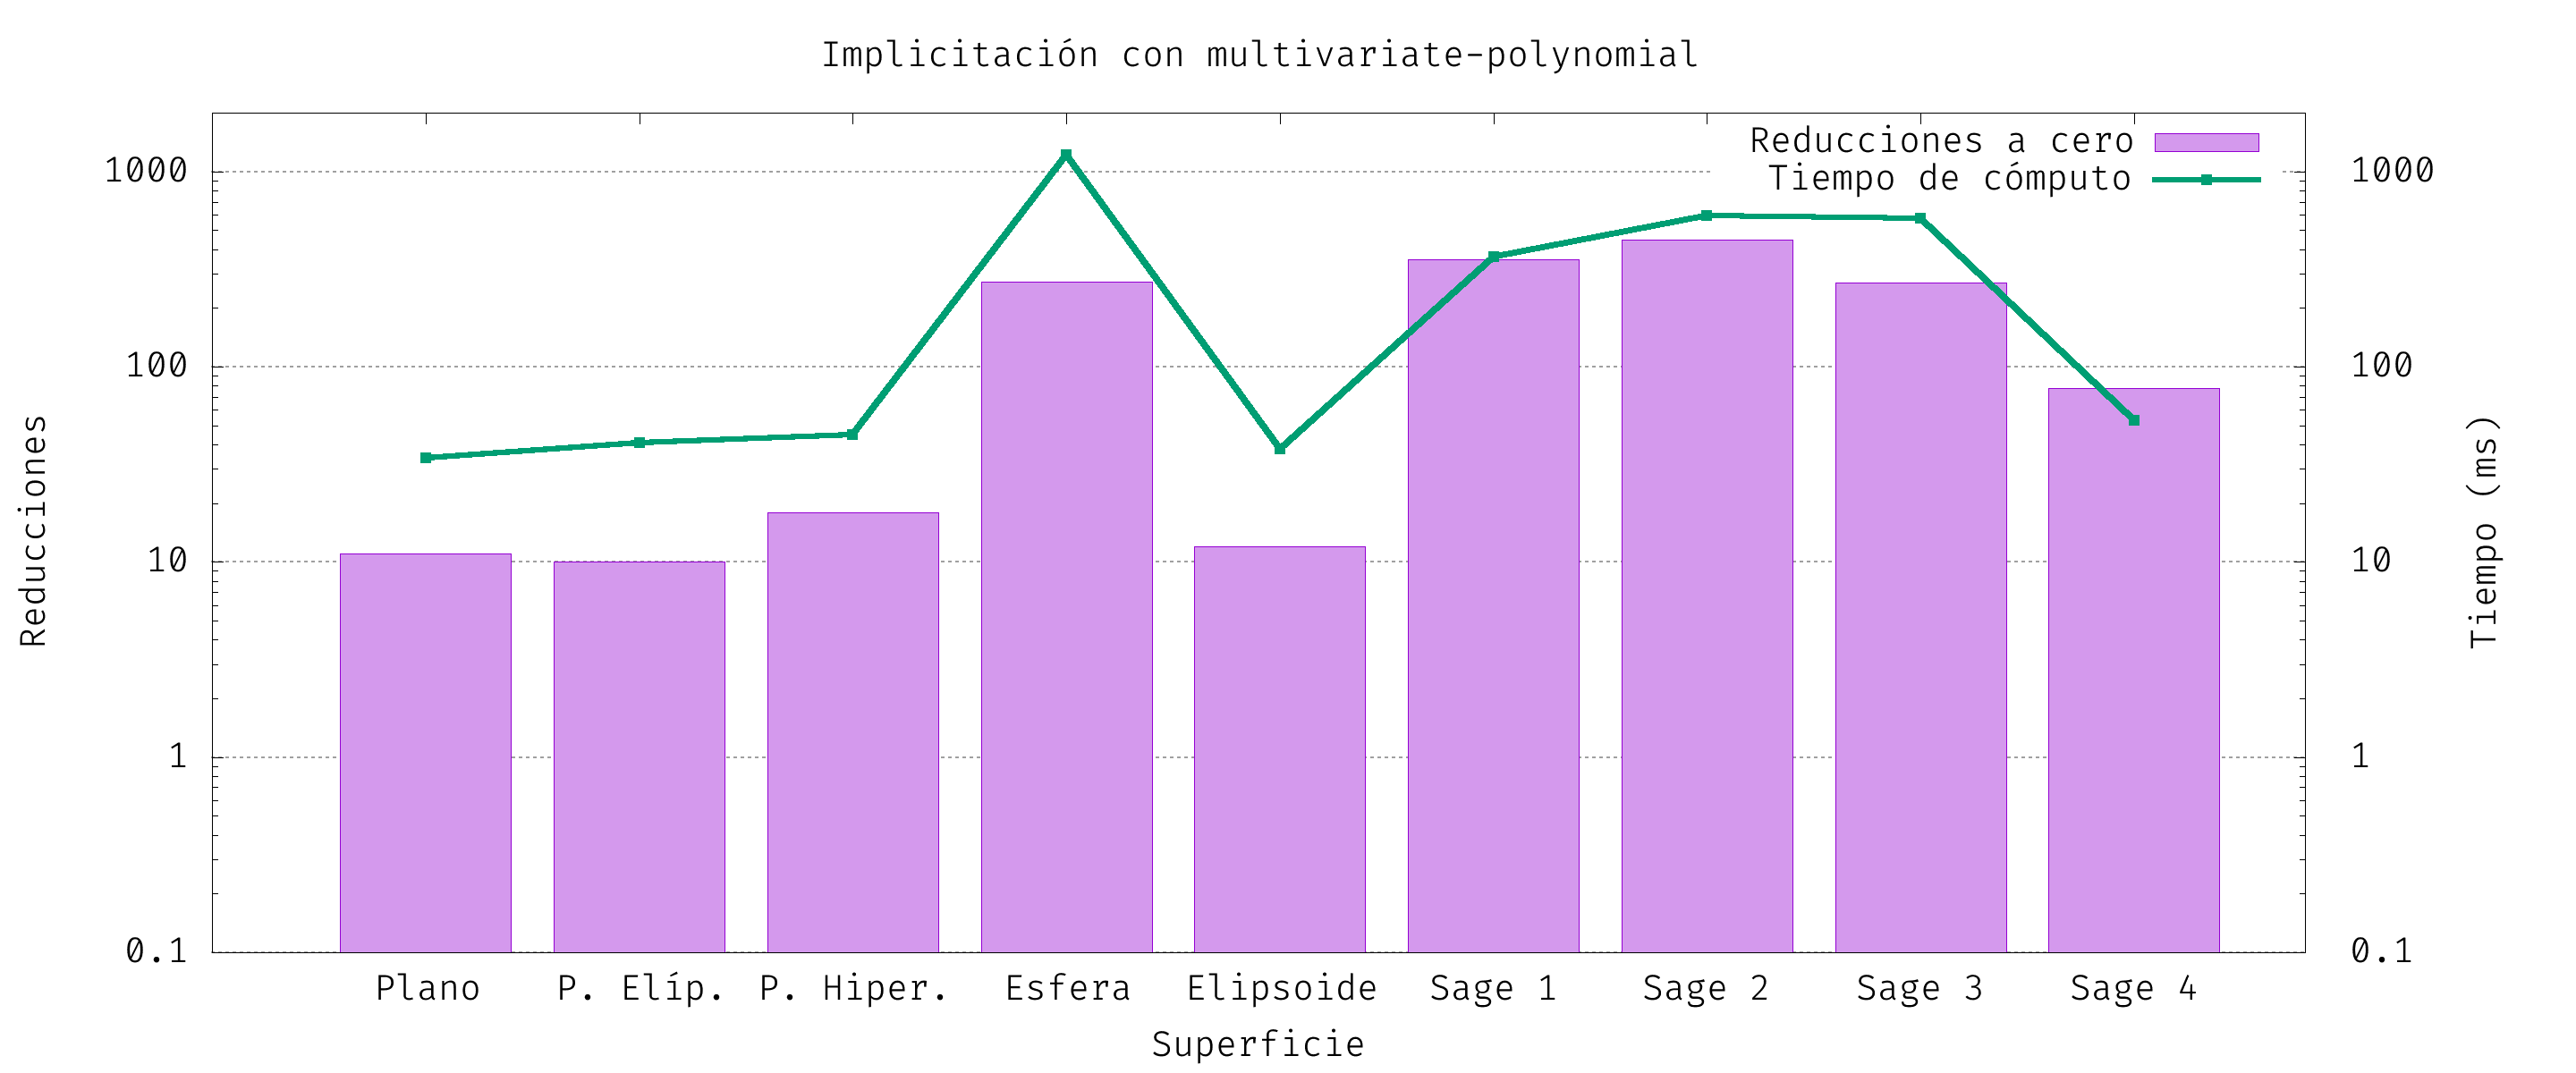
\includegraphics[width=\textwidth]{Plantilla-TFG-master/img/graficas/TiemposImpRed.png}
    \caption{Rendimiento de la implicitación sobre varias parametrizaciones}
    \label{fig:tiemposImpRed}
\end{figure}

Acabamos el capítulo mostrando una comparativa de tiempos entre nuestra librería y Sage, a sabiendas de que obtendremos resultados bastante peores por dos motivos principales.
\begin{enumerate}
    \item Sage es de los \textit{software} de código abierto más completos y optimizados. En concreto, para el cálculo de bases de Gröbner usa Singular, la librería de código abierto más potente en cuanto al cálculo de bases de Gröbner a fecha de realización de este trabajo.
    \item JavaScript no está pensado para optimizar este tipo de cálculos, sino que está diseñado para ejecutarse en navegadores web y brindar interactividad a las páginas web. Además, si bien nuestra versión del algoritmo implementa importantes optimizaciones, esta podría admitir otras que no se han abordado en este trabajo.
\end{enumerate}
El principal objetivo de esta comparación es por tanto ver cómo de cerca hemos conseguido quedarnos respecto a SageMath. En la \autoref{fig:sageVs} vemos que usando \texttt{groebner\_basis}, Sage consigue realizar cada una de las implicitaciones en torno a los 2 ms, siendo estas parametrizaciones en tan solo dos variables muy sencillas para esta versión del algoritmo. Usando  el método \texttt{buchberger}, aún siendo este una versión básica del algoritmo de Buchberger, consigue ser más rápido que nuestra implementación por los motivos mencionados anteriormente, a excepción del caso de la esfera, donde obtiene tiempos similares a nuestra versión.
\begin{figure}[!ht]
    \centering
    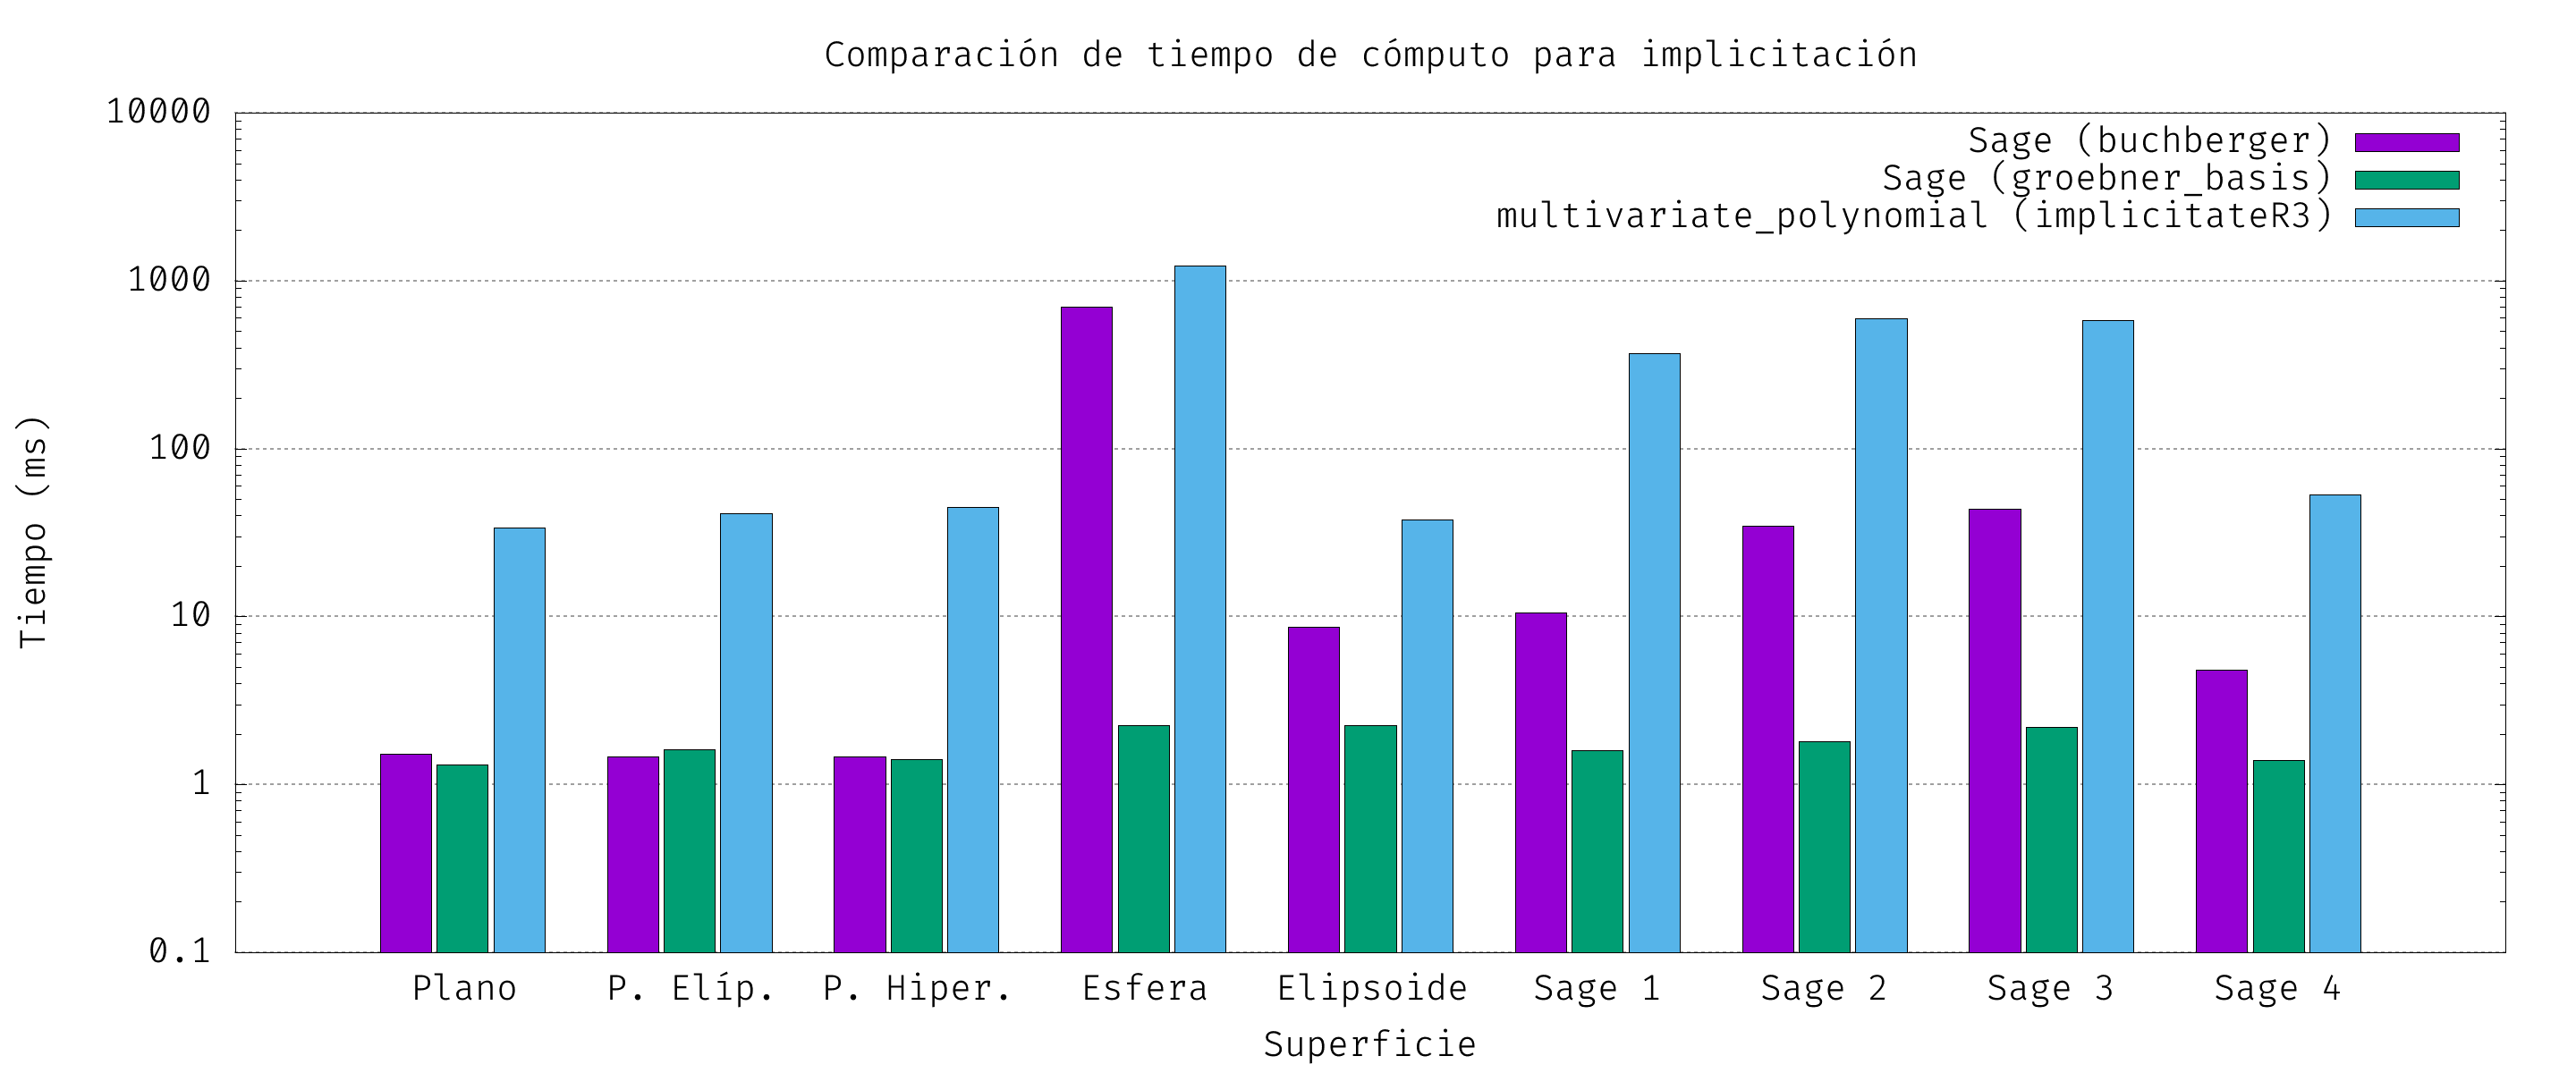
\includegraphics[width=\textwidth]{Plantilla-TFG-master/img/graficas/TiemposImp.png}
    \caption{Comparativa de rendimiento entre Sage y \texttt{multivariate-polynomial}}
    \label{fig:sageVs}
\end{figure}
% Es de esperar que a medida que crezca la complejidad de los generadores o el número de variables, la diferencia de tiempo también aumente. No obstante, los resultados obtenidos 
